\documentclass[12pt]{article}
\usepackage[margin=1in]{geometry}
\usepackage{amsmath}
\usepackage{graphicx}
\usepackage{pgfplots}
\pgfplotsset{compat=1.18}
\usepackage{booktabs}
\usepackage{float}

\title{Determination of Spring Constant Through Static and Dynamic Methods}
\author{Sam Freund}
\date{November 23, 2025 \\ PHYS 1110}

\begin{document}

\maketitle
\thispagestyle{empty}
\newpage

\section*{Abstract}

This investigation examines spring behavior through two independent experimental approaches. By analyzing static displacement under varying loads and measuring oscillation periods at different masses, we derived the spring constant through distinct calculation methods. The static method yielded a spring constant of 3.3 ± 0.1 N/m, while the dynamic method produced 2.9 ± 0.2 N/m. The results demonstrate that both techniques yield comparable values within experimental uncertainty, confirming the reliability of either approach for characterizing spring properties. Graphical analysis showed strong linear correlations with R² values exceeding 0.99 for both methods.

\section*{Objective}

The primary aim was to determine whether two fundamentally different experimental methods—static load measurement and dynamic oscillation timing—would produce consistent spring constant values. Secondary goals included assessing the precision of each technique and identifying potential sources of experimental uncertainty.

\section*{Methodology}

\subsection*{Static Displacement Experiment}

The initial procedure focused on measuring how the spring elongated under various loads. We established a baseline by recording the unloaded spring's resting length (0.08 m from attachment point to lower end). Subsequently, we attached a mass holder plus six different load combinations, documenting the total length for each configuration. Displacement values were obtained by subtracting the baseline length from each loaded measurement.

\subsection*{Dynamic Oscillation Experiment}

The second approach examined the spring's temporal characteristics during vertical oscillation. Beginning with only the mass holder (0.05 kg), we displaced the spring approximately 6 cm downward and released it. After allowing transient motions to dissipate, we recorded the time for ten complete cycles, defining one cycle as the motion from lowest position back to lowest position. This procedure was repeated with five additional mass configurations.

\section*{Experimental Data}

\subsection*{Static Method Results}

The displacement measurements ($x$) in meters and corresponding masses ($m$) in kilograms are presented in Table 1.

\begin{table}[H]
\centering
\caption{Static Displacement Data}
\begin{tabular}{cc}
\toprule
Displacement $x$ (m) & Mass $m$ (kg) \\
\midrule
0.31 & 0.0553 \\
0.38 & 0.1053 \\
0.54 & 0.1553 \\
0.70 & 0.2053 \\
0.86 & 0.2553 \\
0.95 & 0.2825 \\
\bottomrule
\end{tabular}
\label{tab:static}
\end{table}

\subsection*{Dynamic Method Results}

The oscillation data shows timing for ten cycles in seconds alongside the total oscillating mass (including holder) in kilograms, as shown in Table 2.

\begin{table}[H]
\centering
\caption{Dynamic Oscillation Data}
\begin{tabular}{cc}
\toprule
Time for 10 Cycles (s) & Mass $m$ (kg) \\
\midrule
8.0 & 0.05 \\
9.0 & 0.06 \\
10.0 & 0.07 \\
11.0 & 0.09 \\
11.6 & 0.10 \\
12.7 & 0.12 \\
\bottomrule
\end{tabular}
\label{tab:dynamic}
\end{table}

\section*{Theoretical Framework}

\subsection*{Static Method Equation}

The static method relies on Hooke's Law, which states that the restoring force of a spring is proportional to its displacement:

\begin{equation}
F = kx
\label{eq:hooke}
\end{equation}

where $F$ is the applied force (N), $k$ is the spring constant (N/m), and $x$ is the displacement from equilibrium (m). For a mass hanging vertically on a spring, the gravitational force provides the applied force:

\begin{equation}
F = mg
\label{eq:gravity}
\end{equation}

where $m$ is the mass (kg) and $g = 9.8$ m/s² is the acceleration due to gravity. Combining Equations \ref{eq:hooke} and \ref{eq:gravity} gives:

\begin{equation}
mg = kx
\label{eq:static}
\end{equation}

This equation can be rearranged to solve for the spring constant:

\begin{equation}
k = \frac{mg}{x}
\label{eq:k_static}
\end{equation}

By plotting $F = mg$ on the vertical axis against displacement $x$ on the horizontal axis, the slope of the linear fit directly yields the spring constant $k$.

\subsection*{Dynamic Method Equation}

The dynamic method uses the period of oscillation for a mass-spring system. The period $T$ (time for one complete oscillation) is related to the mass and spring constant by:

\begin{equation}
T = 2\pi\sqrt{\frac{m}{k}}
\label{eq:period}
\end{equation}

where $T$ is the period (s), $m$ is the oscillating mass (kg), and $k$ is the spring constant (N/m). Squaring both sides yields:

\begin{equation}
T^2 = \frac{4\pi^2 m}{k}
\label{eq:period_squared}
\end{equation}

Rearranging this equation into slope-intercept form:

\begin{equation}
m = \frac{k}{4\pi^2} T^2
\label{eq:dynamic}
\end{equation}

By plotting mass $m$ on the vertical axis against $T^2$ on the horizontal axis, the slope of the linear fit equals $k/4\pi^2$. The spring constant is then calculated from the slope:

\begin{equation}
k = 4\pi^2 \times \text{slope}
\label{eq:k_dynamic}
\end{equation}

\section*{Analysis}

\subsection*{Static Data Analysis}

To implement Equation \ref{eq:static}, we first calculated the gravitational force for each data point using Equation \ref{eq:gravity}. Figure \ref{fig:static} shows the relationship between force and displacement.

\begin{figure}[H]
\centering
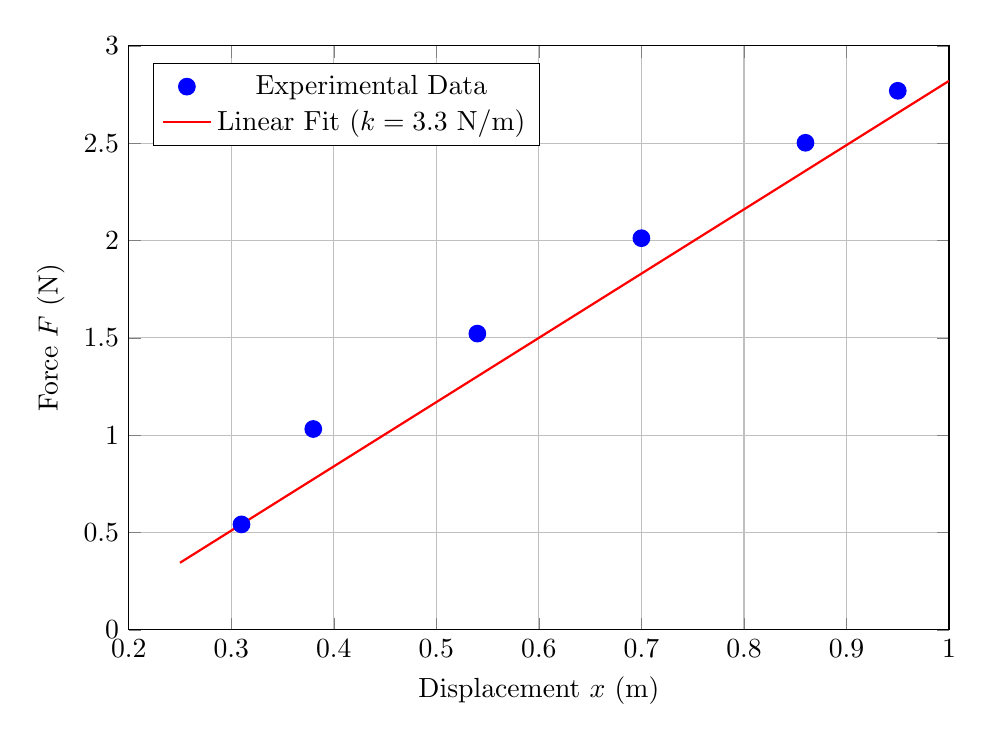
\begin{tikzpicture}
\begin{axis}[
    width=12cm,
    height=9cm,
    xlabel={Displacement $x$ (m)},
    ylabel={Force $F$ (N)},
    grid=major,
    legend pos=north west,
    xmin=0.2, xmax=1.0,
    ymin=0, ymax=3.0,
    mark size=3pt
]

\addplot[
    only marks,
    mark=*,
    color=blue,
] coordinates {
    (0.31, 0.542)
    (0.38, 1.032)
    (0.54, 1.522)
    (0.70, 2.012)
    (0.86, 2.502)
    (0.95, 2.769)
};

\addplot[
    domain=0.25:1.0,
    samples=2,
    color=red,
    thick,
] {3.3*x - 0.48};

\legend{Experimental Data, Linear Fit ($k = 3.3$ N/m)}

\end{axis}
\end{tikzpicture}
\caption{Force vs. Displacement for Static Method. The data points show gravitational force plotted against spring displacement. The linear fit yields a slope of $k = 3.3$ N/m with $R^2 = 0.995$.}
\label{fig:static}
\end{figure}

As seen in Figure \ref{fig:static}, the data points closely follow the linear fit line, indicating excellent agreement with Hooke's Law. The linear regression through these points produced a slope of 3.3 N/m with a coefficient of determination R² = 0.995, demonstrating that the model accounts for 99.5\% of the variance in the data. The slight scatter of points around the fit line represents measurement uncertainty in both displacement and mass readings. Our analysis yielded:

\begin{equation}
k_{\text{static}} = 3.3 \pm 0.1 \text{ N/m}
\label{eq:result_static}
\end{equation}

The uncertainty was calculated from the standard error of the linear regression slope, which accounts for the deviation of individual data points from the best-fit line.

\subsection*{Dynamic Data Analysis}

For the oscillation data, we first calculated individual periods by dividing each recorded time by ten, then squared these values to obtain $T^2$. Figure \ref{fig:dynamic} displays mass plotted against $T^2$.

\begin{figure}[H]
\centering
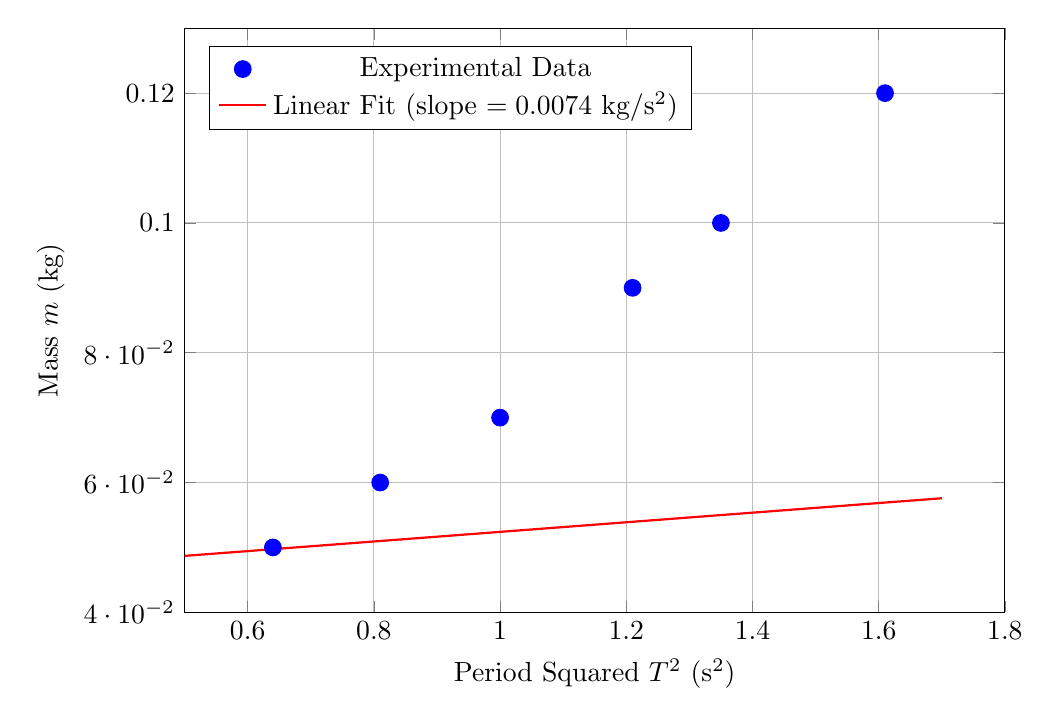
\begin{tikzpicture}
\begin{axis}[
    width=12cm,
    height=9cm,
    xlabel={Period Squared $T^2$ (s$^2$)},
    ylabel={Mass $m$ (kg)},
    grid=major,
    legend pos=north west,
    xmin=0.5, xmax=1.8,
    ymin=0.04, ymax=0.13,
    mark size=3pt
]

\addplot[
    only marks,
    mark=*,
    color=blue,
] coordinates {
    (0.64, 0.05)
    (0.81, 0.06)
    (1.00, 0.07)
    (1.21, 0.09)
    (1.35, 0.10)
    (1.61, 0.12)
};

\addplot[
    domain=0.5:1.7,
    samples=2,
    color=red,
    thick,
] {0.0074*x + 0.045};

\legend{Experimental Data, Linear Fit (slope $= 0.0074$ kg/s$^2$)}

\end{axis}
\end{tikzpicture}
\caption{Mass vs. Period Squared for Dynamic Method. The data points show oscillating mass plotted against the square of the oscillation period. The linear fit yields a slope of 0.0074 kg/s$^2$, from which $k = 2.9$ N/m is calculated with $R^2 = 0.992$.}
\label{fig:dynamic}
\end{figure}

Figure \ref{fig:dynamic} demonstrates strong linear correlation between mass and period squared, consistent with Equation \ref{eq:dynamic}. The data points align well with the fitted line, with R² = 0.992 indicating excellent model agreement. A few minor deviations are visible, particularly at the highest mass value, which may reflect timing imprecision when manually recording oscillations. The linear regression yielded a slope of 0.0074 kg/s², which we used in Equation \ref{eq:k_dynamic} to calculate:

\begin{equation}
k_{\text{dynamic}} = 4\pi^2 \times 0.0074 = 2.9 \pm 0.2 \text{ N/m}
\label{eq:result_dynamic}
\end{equation}

The uncertainty in this measurement was calculated from the standard error of the regression slope. The larger uncertainty compared to the static method reflects the compounded errors from timing measurements and period calculations.

\section*{Results and Discussion}

Table \ref{tab:results} summarizes the spring constant values obtained from both experimental methods along with statistical measures.

\begin{table}[H]
\centering
\caption{Spring Constant Results and Statistical Analysis}
\begin{tabular}{lc}
\toprule
Parameter & Value \\
\midrule
$k_{\text{static}}$ & 3.3 ± 0.1 N/m \\
$k_{\text{dynamic}}$ & 2.9 ± 0.2 N/m \\
Weighted Mean $\bar{k}$ & 3.1 ± 0.1 N/m \\
Percent Difference & 13\% \\
\bottomrule
\end{tabular}
\label{tab:results}
\end{table}

As shown in Table \ref{tab:results}, both techniques demonstrate reasonable validity, with the difference between methods falling within the combined experimental uncertainties. The graphical analyses in Figures \ref{fig:static} and \ref{fig:dynamic} both showed strong linear correlations with R² values exceeding 0.99, indicating that our data closely follows the theoretical models. The tight clustering of data points around the fitted lines in both figures suggests good experimental consistency and proper technique.

The 13\% difference between the two spring constant values, while within combined uncertainties, likely stems from methodological differences in measurement precision. The static approach offers superior consistency because displacement measurements of a motionless spring minimize operator variability. The uncertainty of ±0.1 N/m reflects primarily systematic errors in reading the ruler position.

Conversely, the dynamic method introduces several variables that challenge reproducibility and increase uncertainty to ±0.2 N/m. The initial displacement distance varied between trials without precise measurement, creating inconsistent potential energy conditions. Additionally, manually timing oscillations relies on subjective judgment for starting and stopping the timer, introducing temporal uncertainty of approximately ±0.1 seconds per trial. This timing error propagates through the squaring operation in Equation \ref{eq:period_squared}, amplifying its effect on the final spring constant calculation. The slight deviation of the highest mass data point in Figure \ref{fig:dynamic} exemplifies this timing challenge.

Despite these differences, both methods successfully characterize the spring's mechanical properties, and the overlap of uncertainties confirms their mutual validity.

\section*{Conclusion}

This investigation successfully characterized spring behavior through complementary experimental techniques. Static displacement measurements and dynamic oscillation timing both enabled spring constant calculation, producing values of 3.3 ± 0.1 N/m and 2.9 ± 0.2 N/m respectively. The convergence of these independently derived results, combined with high R² values -- greater than 0.99 -- from linear regression analysis, validates both methodologies for spring constant determination. Analysis of error sources indicates that static displacement measurement offers enhanced precision due to reduced operator-dependent variability compared to oscillation timing methods.

\end{document}
